%\documentclass[11pt]{article}
\documentclass[preprintnumbers,prd,superscriptaddress,notitlepage,nofootinbib] {revtex4-1}

\usepackage{geometry, amsmath, amsthm, latexsym, amssymb, graphicx}
\geometry{margin=1in, headsep=0.25in}
\usepackage[usenames, dvipsnames]{color}

%comments by co-authors
\newcommand{\AFR}[1]{{\color{red}AFR: #1}}

%journals
\newcommand{\mnras}{{\em Mon. Not. Roy. Astron. Soc. }}
%\newcommand{\apj}{{\em Astrophys. Jour. }}
%\newcommand{\apjl}{{\em Astrophys. J. Let. }}
\newcommand{\apjs}{ApJS}
\newcommand{\jcap}{JCAP}
%\newcommand{\physrep}{{\em Phys. Rept. }}
\newcommand{\aap}{{\em Astron. Astrophys. }}
%\newcommand{\prd}{{\em Phys. Rev.}}
%\newcommand{\aj}{AJ }

%others
\newcommand{\lya}{Ly-$\alpha$}
\newcommand{\kms}{{\rm km~s^{-1}}}  
\newcommand{\ikms}{{\rm s~km^{-1}}}
\newcommand{\iMpc}{{\rm Mpc^{-1}}}
\newcommand{\kpar}{k_\parallel}
\newcommand{\Plin}{P_{\rm lin}}

\begin{document}

\title{Parameterization of the \lya\ forest power spectrum}

\author{Andreu Font-Ribera \footnote{author list alphabetized}}
\email{a.font@ucl.ac.uk} 
\affiliation{Department of Physics and Astronomy, University College London, 
Gower Street, London, United Kingdom}
\author{Patrick McDonald}
\email{PVMcDonald@lbl.gov} 
\affiliation{Lawrence Berkeley National Laboratory, One Cyclotron Road,
Berkeley, CA 94720, USA}
\author{An\v{z}e Slosar}
\email{anze@bnl.gov} 
\affiliation{Brookhaven National Laboratory, Upton, NY 11973, USA}

\date{\today}

\begin{abstract}
Discuss unique role of \lya\ forest power spectrum, running and neutrino mass.
Discuss the need of emulators and expensive hydrodynamical simulations, and
the critical choice of likelihood parameterization.
Mention BOSS, eBOSS, DESI and high-resolution spectra.
\end{abstract}

\maketitle

\section{Introduction} 

Discuss here the unique window opened by Lyman-$\alpha$ (\lya) forest 
clustering, to study the linear power spectrum on small scales and redshifts 
higher than those available from galaxy surveys.
Discuss the role of hydrodynamic simulations in these studies, and the need 
for an emulator.
Discuss the importance of chosing the right parameterization in the emulator, 
since some cosmological parameters are not well measured by the \lya\ forest.
In particular, mention neutrino-mass degeneracy and the reasons to not use 
$\sigma_8$ defined at redshift zero.

Mention that even though this was studied already in \cite{McDonald2005a}, 
recent papers have ignored this issue \cite{Palanque-Delabrouille2015,
Yeche2017}. 
This will be relevant for future analyses, specially from DESI.

Even though past analyses have focused on the 1D power spectrum, 
the 3D power spectrum can also be measured \cite{Font-Ribera2018}, 
and it contains most of the information available from future surveys 
like DESI \cite{Font-Ribera2014}. 

In this paper we take another look at this topic, using modern hydrodynamic 
simulations and explicitely showing the accuracy of some of the approximations.
We start in section \ref{sec:over} with an overview of the different steps 
involved in a cosmological inference from the \lya\ power spectrum, and we 
continue in \ref{sec:like} with a description of the likelihood code, 
its user interface, and its internal parameterization. 
We describe the link between the likelihood and the \textit{emulator} in
section \ref{sec:emu}.
In section \ref{sec:sims} we discuss the simulations used in the emulator, 
and the post-processing of the snapshots. 
 


\section{Cosmological analyses with the \lya\ forest power spectrum}
\label{sec:over}

In this section we present an overview of the different aspects involved in 
a cosmological analysis of the small scale clustering from the \lya\ forest
power spectrum.

\begin{itemize}
 \item Measurement of the flux power spectrum: calibrate the quasar spectra, 
  fit the quasar continua, measure 2-point functions, covariance matrices 
  and possible contaminants.
 \item \textit{Emulate} the flux power spectrum: using hydrodynamical 
  simulations, build an emulator to translate the measured flux power to 
  constraints on the linear power spectrum of density at the redshift of 
  the measurement ($z \sim 3$).
 \item Cosmological constraints: combine the inferred linear power spectrum
  with external datasets (primarily CMB studies) to constraint the parameters
  of a particular cosmological model.
\end{itemize}


\subsection{Measuring the \lya\ correlations}

Skip over continuuming fitting, instrumental details, and so on.
This will not be the main focus of this paper.

\begin{figure}[h]
 \begin{center}
  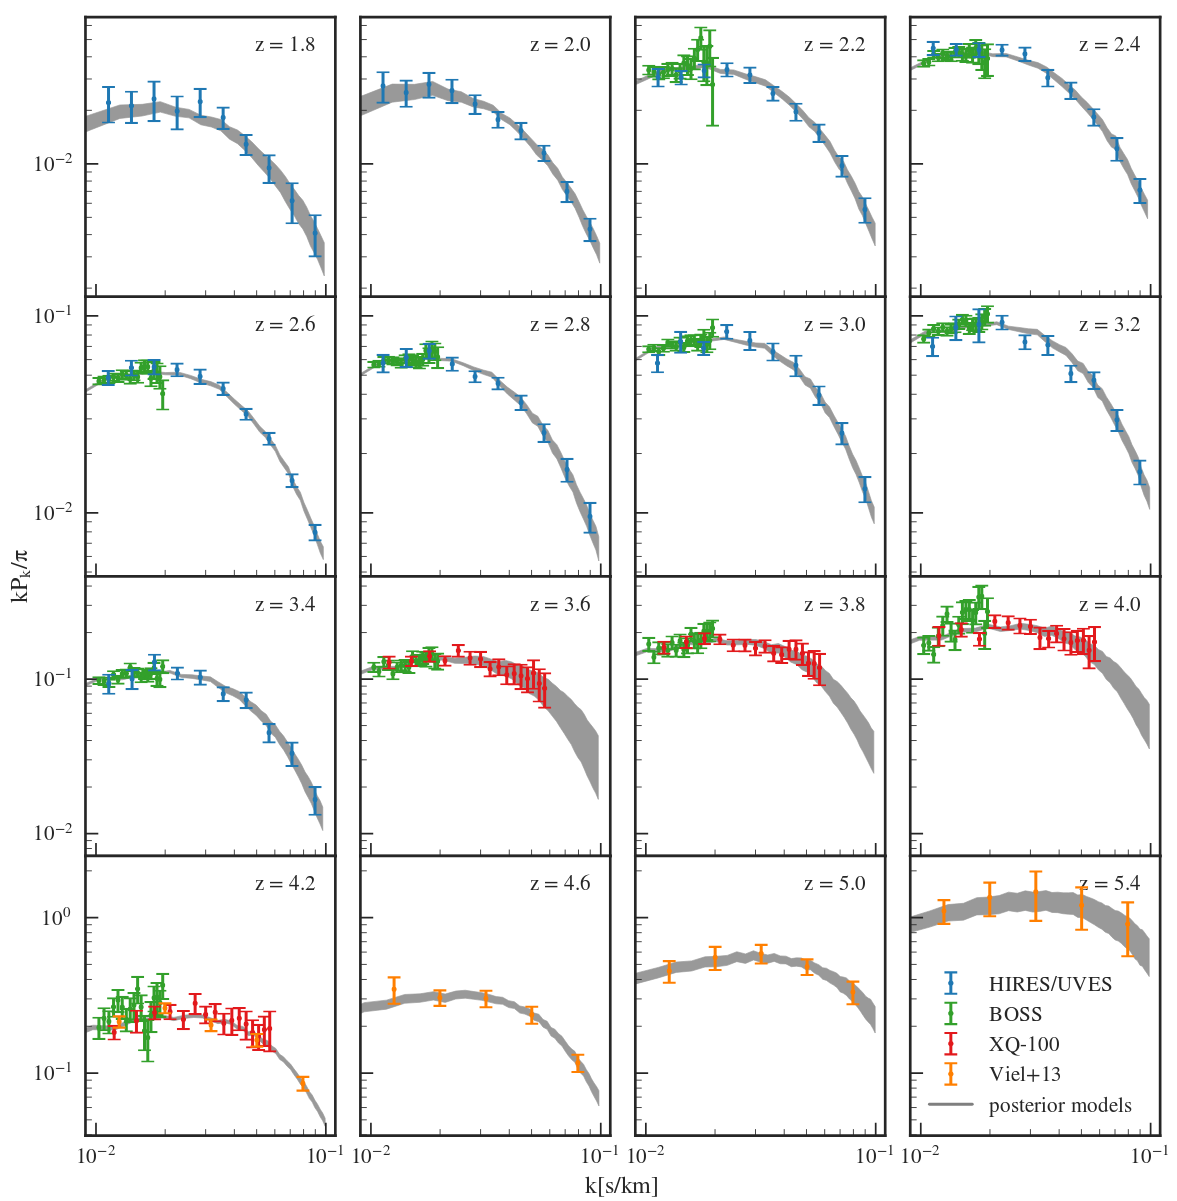
\includegraphics[scale=0.34]{Figures/Walther2018_P1D}
  %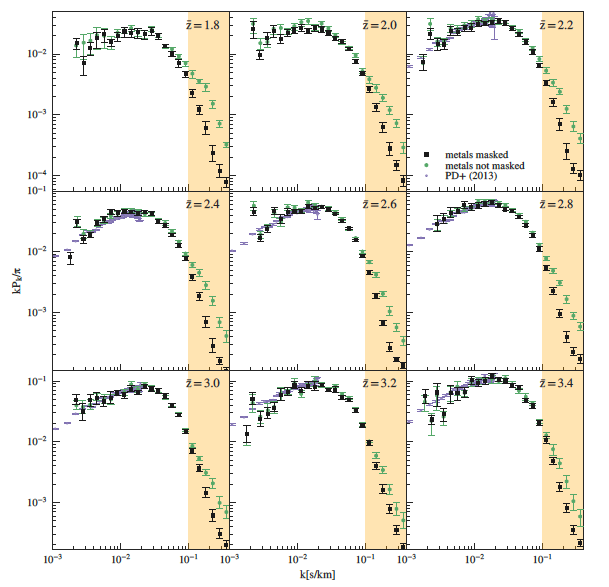
\includegraphics[scale=0.6]{Figures/WaltherP1D}
 \end{center}
 \caption{Compilation of $P_{1D}(z,\kpar)$ measurements, including those from
  \cite{Viel2013} (orange), \cite{Irsic2017} (red), 
  \cite{Palanque-Delabrouille2013} (green) and \cite{Walther2018a} (blue). 
  \AFR{This figure was stolen from \cite{Walther2018b}, it would be better to 
  add one that goes to lower values of $\kpar$ covered by SDSS/BOSS.}
 }
 \label{fig:dataP1D}
\end{figure}

Beyond BAO analyses \cite{Bautista2017,duMasdesBourboux2017}, the only 
public results on the clustering of the \lya\ forest are measurements of 
the 1D power spectrum \cite{Croft1998,McDonald2000,McDonald2006} or 
more recently \cite{Viel2013,Palanque-Delabrouille2013,Irsic2017,Walther2018a}.
These are usually presented as band powers measured in different redshift
bins, spanning the redshift $1.8 < z < 5.4$, and covering a broad range of 
scales $0.001 \ikms < \kpar < 0.1 \ikms$. 
A compilation of recent measurements is shown in Figure \ref{fig:dataP1D}.

In most cases, the line of sight wavenumbers are expressed in units of 
inverse velocity, $\ikms$, but other mappings from observed wavelength 
could be used.
When measuring the 3D power, we will also need to define transverse 
wavenumbers, and in this case the natural choice is to use units of 
inverse angles \cite{Font-Ribera2018}.


\subsection{\textit{Emulating} the flux power spectrum}

In order to interpret the measurements, we need to be able to make 
theoretical predictions for the measured correlations, and setup a statistical 
method to compare models and compute constraints on their parameters.  

Due to its non-linear nature, to simulate the \lya\ forest (or flux) power 
spectrum we need to rely on expensive hydrodynamical simulations. 
Each model evaluation requires thousands of CPU hours, what makes a 
\textit{brute-force} approach unfeasible. 

Moreover, the flux power spectrum does not only depend on the density 
clustering, but it also depends on the thermal history of the 
Inter-Galactic Medium (IGM) (see \cite{Walther2018b} for a recent review).
In order to compute robust cosmological constraints, we need to make sure 
that we explore all possible thermal histories, and that we fully marginalize 
over these nuisance parameters.

This large parameter space, and the cost of a single run, makes it impossible 
to run a simulation for each model we want to compare.
A small number of simulations is usually available, and in the past different 
analysis have used different techniques to circumvent this problem: 
a smooth dependence was assumed and fit in \cite{McDonald2005a}; 
a Taylor expansion was used in \cite{Palanque-Delabrouille2013}; 
a Gaussian Process-based \textit{emulator} was used in 
\cite{Walther2018a,Walther2018b}, although in this analysis the cosmological
model was kept fixed and only the thermal history was explored.

Emulators based on Gaussian Processes are an active area of research 
\AFR{cite density emulators}, and it is possible that they will have an 
important role in future \lya\ forest analyses.
However, in this publication we will use the term \textit{emulator} in a broad
sense, to describe any setup to use a finite suite of hydrodynamical 
simulations to make predictions for the flux power spectrum.

The main topic of this paper is to study the parameter degeneracies in this 
type of analyses, and discuss how this might affect the parameterization of 
an emulator for the flux power spectrum.


\subsection{Cosmological constraints}

As we will discuss in the next sections, once we have marginalized over 
the thermal history of the IGM, the flux power spectrum is mostly 
sensitive to the amplitude and slope of the linear power spectrum around 
$k \sim 1 \iMpc$ 
\footnote{As it will be discussed in the next sections, the pivot point 
should be specified in velocity units, $k \sim 0.01 \ikms$.} 
and around $z \sim 3$.
For instance, \cite{McDonald2005a} measured these quantities with 15\% and 
5\% precision respectively.

Changes in other (traditional) cosmological parameters are very degenerate 
with changes in the linear power or in the thermal history. 
For instance, as discussed in \cite{Viel2010} and more recently in 
\cite{Pedersen2018}, at fixed linear power spectrum the effect of massive 
neutrinos is almost indistinguishable from that of $\Omega_m$. 
Another exmaple: at fixed linear power spectrum, and fixed $\Omega_m$, the 
effect of $\Omega_b$ is degenerate with the level of UV background assumed.

One of the peculiarities of \lya\ forest analyses that we will discuss is 
that it covers a redshift range $2 < z < 5$ where the universe was close 
to Einsteint-de Sitter (EdS), i.e., $\Omega_m(z) \sim 1$. 
This means that the growth of structure in this redshift range is almost  
independent of cosmology, and so is the expansion history $H(z)/H_0$.

It is only in combination with external datasets, mainly from CMB experiments,
that we are able to provide constraints on the traditional cosmological 
parameters. 
For instance, by combining our measurement at $k \sim 1 \iMpc$ with the CMB 
constraints on the amplitude and slope of the linear power spectrum at 
$k \sim 0.05 \iMpc$ we get tight constraints on the running of the spectral
index ($\alpha_s$) and on the sum of the neutrino masses ($\sum m_\nu$). 

This approach of emulating only the linear power was used in 
\cite{McDonald2005a}, but recent analyses 
\cite{Palanque-Delabrouille2015,Yeche2017} have attempted instead to 
directly emulate the 6+ traditional parameters of a $\Lambda$-CDM universe. 
We will argue that this might not be the best approach, because of the
following reasons:
\begin{itemize}
 \item As discussed above, the traditional parameters have strong degeneracies
  and this makes the emulator (or Taylor expansion) more challenging. 
 \item In order to break the degeneracies, one needs to adopt priors from 
  CMB experiments, making it more dificult to combine with CMB experiments 
  later without double counting information.
 \item The results are model-dependent, and it is impossible to use them in 
  extended models (curved universe, non-$\Lambda$, different $N_{\rm eff}$...)
  if these were not in the original emulator.
\end{itemize}


\section{Public likelihood code}

In order to properly discuss our choice of parameterization and simulation
setup, it is important to describe how we intend the end product,
the \textit{likelihood code}, to be used in a cosmological analysis.


\subsection{User interface}

The aim of the project is to provide a public likelihood package that others
can use to include \lya\ results in their cosmological parameter constraints.
The end-user does not need to know about the internal details, about the 
suite of simulations, the nuisance parameters or the interpolation scheme 
used in the emulator.
They do not need to know either whether internally we are describing the 
power in units of $\kms$, $\Mpc$ or $\hMpc$. 

There are different possible interfaces that we could setup, and probably 
we will want to provide more than one with different levels of complexity.
But we will start discussing a particular interface, where we will ask 
the user to provide for each cosmologicla model:
\begin{itemize}
 \item Linear matter power (baryons+CDM), as a function of redshift and 
  wavenumber, in units of $\iMpc$. 
  The redshift range should cover at least $2 < z < 5$, and the wavenumber
  range should cover at least $0.01 \iMpc < k < 10 \iMpc$. 
  For simplicity, we will restrict ourselves to models with a linear power 
  spectra that can be factorized ,in the range of redshift and scales 
  described above, in a power spectrum at a central redshift, 
  $P_L(z_\star=3,k)$, and a scale independent growth factor, $D(z)$.
 \item Logarithmic growth rate, $f(z)$, that could be computed directly
  from the evolution of $D(z)$.
 \item Hubble parameter as a function of redshift, $H(z)$, over the same 
  redshift range.
 \item If we want the likelihood code to be able to fit 3D clustering as well,
  we would need as an input the angular diameter distance, $D_A(z)$, 
  over the full redshift range.
\end{itemize}

The user will also specify:
\begin{itemize}
 \item Data products to use: 
  SDSS-I from \cite{McDonald2006}, 
  BOSS from \cite{Palanque-Delabrouille2013},
  HIRES/UVES from \cite{Viel2013},
  XQSO-100 from \cite{Irsic2017}, 
  HIRES/UVES from \cite{Walther2018a}. 
  We should also allow the user to specify what redshifts to use from each
  dataset, since they are independent, and probably also allow the user 
  to specify the scales to be used in the fit for each dataset.
 \item Extra analysis settings, like whether to allow for running in the 
  linear power, non-EdS linear growth...
 \item \AFR{It is not clear to me whether at this point the user would also
  be able to set other settings of the likelihood or not, like the way we 
  treat contamination by DLAs or metals, resolution or noise corrections, 
  or the parameterization of the temperature-density relation in the 
  simulations.}
 \item \AFR{I guess the user should also be able to specify priors for
  the parameters that we want to marginalize over. 
  We could even provide the option to use published temperature / mean flux
  results as a prior on thermal history and mean flux, although this should 
  be an option that would be switched off by default...}
\end{itemize}

The output from the \textit{likelihood code} will be:
\begin{itemize}
 \item A value of (log-)likelihood for each dataset, possibly a value for 
  each redshift bin. 
  Most users will only care about this.
 \item For the experts, we would also output the best-fit theoretical 
  prediction for each dataset, for that particular cosmological model.
  We would also provide the values of the nuisance parameters that correspond
  to the best fit model (mean flux, temperature-density relation, metal or DLA
  contamination...).
 \item We could also provide a random sample of theory lines that are above a 
  likelihood threshold for that particular model, exploring different 
  thermal histories and other nuisance parameters.
\end{itemize}


\subsection{From cosmological model to emulator input}

Under the hood, we will use more effective (and cryptic) parameters in our 
\textit{emulator}, understood as the package that will use black magic 
(or white magic) and a suite of hydrodynamical simulations to make 
predictions for the flux power spectrum.

There are many, many possibilities here, but we will start by discussing a 
possible setting. 

\begin{itemize}
 \item We will choose a fiducial cosmological model, based on a recent 
  Planck+BAO analysis, and use it to compute a fiducial linear power spectrum,
  $P_L^0(z,k)$, a fiducial Hubble expansion, $H^0(z)$, a fiducial growth 
  rate $f^0(z)$...
 \item We will compress the difference between the input power spectrum, 
  and the fiducial power spectrum, into a handful of parameters. 
  Probably this would include the sound horizon at the drag epoch, setting 
  the scale of the Baryon Acoustic Oscillations (BAO), $r_d$, and 3 extra 
  parameters describing the smooth differences in the broadband.
  We would ignore differences between baryons and CDM, and always work with 
  their weighted-averaged power. 
  We will fit these parameters using the linear power at a central redshfit,
  $z_\star=3$, but since we have decided to use only models where the 
  linear power spectrum can be factorized, this should not have an impact.
 \item We will compute the ratio of the input growth rate with that in the 
  fiducial cosmology, $R_f = f(z_\star)/f^0(z_\star)$, evaluated at 
  $z_\star=3$. 
  We will approximate that the growth rate at $z_\star$ is enough to compute 
  the linear power at any redshift within the range:
  \begin{equation}
   P_L(z_\star+\Delta z,k) = P_L(z_\star,k) \left[ 1 
      - 2 \frac{f(z_\star)}{(1+z_\star)} \right] ~. 
  \end{equation} 
  \AFR{I haven't cross-checked the equation above, but you got the idea.}
  \AFR{I'm not sure this is the best idea, probably better to use the 
   redshift evolution of the fiducial cosmology, and only a small correction
   using $R_f$.}
\end{itemize}

If we could observe the \lya\ power spectrum in comoving coordinates, that 
would be enough. 
However, we observe the power spectrum in observing coordinates, wavelengths
and angles, and a more natural choice is to use velocity units ($\kms$) for 
the clustering measurements. 
Indeed, all recent measurements of the 1D \lya\ power reported their results
in units of $\kms$, and we will assume the same in this discussion.






\section{Degeneracies in linear theory}
\label{sec:lin}

Discuss the degeneracies in the context of linear theory, using model
predictions from CAMB.




\section{Simulations}
\label{sec:sims}

Describe here the simulations, include the initial conditions code (GenIC), 
the code to evolve the fields (MP-Gadget), the different boxes used, 
and the code to extract skewers (fake\_spectra).

Discuss also here the optical depth rescaling, different transfer functions
(if any), and thermal history effects (that will be mostly ignored in this
paper).


\subsection{Rescaling of the optical depth}

From each simulation we will get a set of snapshots, outputs at different 
redshifts. 

From each snapshot, we will extract \lya\ skewers, and use these to compute 
their power spectra. 
We will repeat this exercise for different rescalings of the optical depth, 
i.e., we will multiply the optical depth in all cells by a constant factor
in the range $0.8 < A_\tau < 1.2$ (approximately), and for each value of 
$A_\tau$ we will compute the transmitted flux fraction $F$, its mean value
(mean flux), and the power spectra of their fluctuations $\delta_F$. 

Therefore, from each snapshot we will get a set of power spectra for different
values of $A_\tau$.
We can label the different power spectra by their associated value of $A_\tau$,
or we can label them by their resulting value of the mean flux $\bar F$. 

\cite{Lukic2015} showed that the rescaling might introduce biases in the 
1D power spectrum for values of $A_\tau$ very different than one. 
However, their test compared two simulations with different thermal history
and different pressure, so it is difficult to tell whether the bias came 
from the rescaling or from the different IGM physics.

\AFR{It would be great to repeat this exercise in two simulations that 
have very similar thermal history but different mean flux, I will ask 
Jose Onorbe for help (he is visiting UCL soon). 
It is also possible that the test is clearer if we look at the 3D power,
where pressure only affects the high-k limit, and the scale independent
linera bias.}


\subsection{Rescaling of the temperature}

The Temperature-Density Relation (TDR) in the \lya\ forest can be reasonably
well described by a power law, 
\begin{equation}
 T(\rho) = T_0 \left(\frac{\rho}{\rho_0}\right)^{\gamma-1} ~,
\end{equation}
with a typical values for $\gamma$ between 1 and 1.6. 
If we use $\rho_0 = \bar \rho$, $T_0$ varies between 10,000 and 20,000K
\cite{Lukic2015}.

We can change the thermal history of the simulations by running the same box
with different \textit{TREECOOL} files, that contain the redshift evolution
of different heating and ionizing rates.

For each snapshot, we can fit their values of $T_0$ and $\gamma$, and use 
these to label the snapshot, instead of using the name of the TREECOOL, 
or the parameters that we have used to modify a given file 
(MP-Gadget can implement the recipes in \cite{Bolton2008} to modify TRECOOL
files by setting the parameters \textit{HeatAmplitude} and \textit{HealSlope}).

Just like we did with the optical depth, we can rescale the temperatures in 
post-processing. 
We could do this at two different levels:
\begin{itemize}
 \item Thermal broadening: when extracting the skewers from the boxes, 
  the last step is to compute the redshift-space-distorted optical depth. 
  To do that, the temperature at each cell is used to decide the local 
  smoothing that we need to apply, what is known as the thermal broadening. 
  It is trivial to take the same optical depth skewer, and convolve it for
  different temperature rescalings.
 \item Recombination rates: the temperature also sets the recombination rate,
  $\alpha(T) \sim T^{-0.7}$. 
  It would also be possible to change the recombination rate at each cell, 
  propagate this into a change in the neutral fraction (proportional to the 
  recombination rate), and finally to the optical depth (proportional to the 
  neutral fraction). 
\end{itemize}

Note that, even though this would capture most of the effects of having a 
different temperature, we would miss the effect that different temperature
have in the pressure smoothing.
However, we will include a parameter to study the dependence on the pressure
smoothing, the filtering length $k_F$, and this should be able to capture
the differences.


\subsection{Adding pressure smoothing}

The small scale structure is suppressed on very small scales because of the
pressure in the gas. 
As described in \cite{Hui1997,Gnedin1998}, the smoothing can be described
by a characteristic scale, $k_F(z)$, the \textit{filtering scale}, that is
an integral version of the Jeans length that depends also on the temperature
in the past.

It would be interesting to see if we can add smoothing in postprocessing, 
effectively lowering the value of $k_F$ in the simulation by hand. 
Of course, it would not be possible to reduce the smoothing, and to do that 
one would need to run a simulation with an earlier redshift of reionization.

\AFR{We could also ask Jose Onorbe for help to setup this type of test. 
We would also need to discuss the best way to measure $k_F$ in the snapshots:
fit a Gaussian kernel in the power spectrum of $F_{\rm real}$, where no 
redshift-space distortions have been included? I believe that is what is 
used in all papers by Hennawi / Lukic / Onorbe.}


\subsection{Labelling the snapshots}

In the linear regime, and for a single specie, the growth of structure is 
scale independent, and it can be described by the growth factor $D(z)$.
%\begin{equation}
% P_L(z,k) = \frac{D^2(z)}{D^2(z_0)} ~ P_L(z_0,k) ~.
%\end{equation}

If the \lya\ power spectra depended only on the linear power spectrum, this 
would suggest that there would be a complete degeneracy between changing 
the overall amplitude of the linear power spectrum and changing the redshift
at which we ouput the snapshot. 
Therefore, we could use the amplitude of the linear power at a given snapshot
to label it, and use the different snapshots of the same simulation to study 
models with different amplitudes of the linear power. 

In section \ref{sec:dens} we will check whether this is still true at the 
level of the non-linear power spectrum, and in section \ref{sec:lya} we 
will look at this degeneracy in the \lya\ power spectrum. 

\AFR{How do we measure the linear power in the snapshot? 
I could see three options (in order of my preference): 
predict it using the power measured in the initial conditions, and the relative
growth as computed from CAMB/CLASS;
measure the density power in the snapshot, and fit the growth factor from 
the low-k part;
run a very cheap simulation without hydro and a very low value of $A_s$, to 
compute the actual linear power in the simulation (that might sadly differ 
from the predicted by CAMB/CLASS because of issues in the linear growht).}

To sum up, each snapshot will be used to generate multiple simulated 
fields, and we can label each of them by their values of: 
mean flux (1 parameter) $\bar F$,
linear power (3 parameters) $P_L$,
TDR (2 parameters) $T_0$ and $\gamma$, 
filtering scale $k_F$.

Redshift will NOT be a label describing the simulated field, and neither
will be the TREECOOL file or the redshift of reionization.
Since we will define the linear power in units of $\kms$, we will not 
need to include the Hubble parameter at the box as a label.
We will not care about any other cosmological parameter in the box
either.


\section{Degeneracies in the non-linear density power spectrum}
\label{sec:dens}

Use the simulations to measure the non-linear power spectrum of density
fluctuations, and show that the degeneracies are still there.


\section{Degeneracies in the flux power spectrum}
\label{sec:lya}

Show here the degeracies in the \lya\ 1D power (may be also 3D).



\section{Discussion}
\label{sec:disc}

Add here the discussion, and future work.


\section*{Acknowledgements}
AFR acknowledges support by an STFC Ernest Rutherford Fellowship, grant reference ST/N003853/1.
AS acknowledges hospitality of the University College London.
This work was partially enabled by funding from the UCL Cosmoparticle
Initiative.

\bibliography{main}
\bibliographystyle{JHEP}

%\appendix


\end{document}
